\documentclass{article}
\usepackage{verbatim}
\usepackage[utf8]{inputenc}
\usepackage[russian]{babel}
\usepackage{graphicx}

\begin{titlepage}
  \title    {Элементы документации к задаче 32}
  \author   {Маллабаев Азамат Нурмухамадович}
  \date     {2015}
\end{titlepage}

\begin{document}
  \maketitle
  \section{Требования}
  \subsection{Зачем}
    Сравнить скорость вычисления чисел Фиббоначи в разной арифметике
  \subsection{Сценарий}
  \begin{enumerate}
    \item Построить график зависимости (в виде ломанной) времени выполнения
    \item Сделать выводы
  \end{enumerate}
  \subsection{Функции}
  \begin{enumerate}
    \item Каждая реализация вычислителя для 0 и 1 выдает 0 и 1, соответственно
    \item Каждая реализация вычислителя для двух последовательных чисел выдает в качестве третьего их сумму
    \item Функция времени от n - возрастающая, чтобы избежать скачков и легко было аппроксимизировать
  \end{enumerate}
  \pagebreak
  \section{Тесты}
  \subsection{Зачем}
    Собрать статистику и решить, какой алгоритм наиболее удачен для данных значений аргумента
  \subsection{Сценарий}
  \begin{enumerate}
    \item Запросить ввод числа k
    \item Для каждой реализации вычислителя:
    \begin{enumerate}
      \item Для каждого n с -k по k посчитать
      \begin{itemize}
        \item n-ое число Фибоначчи
        \item Посчитать время вычисления этого числа
      \end{itemize}
      \item Построить график зависимости (в виде ломанной) времени выполнения от n на промежутке от -k до k
    \end{enumerate}
  \end{enumerate}
  \subsection{Функции}
  \begin{verbatim}
    Функциональный тест 1
    val ft1: (num -> Tot num) -> Tot unit
    let ft1 f = assert((f 0 = 0) && (f 1 = 1))

    Функциональный тест 2
    val ft2: (num -> Tot num) -> num -> Tot unit
    let ft2 f x = assert(f x = (f (x + 1) + f (x + 2)))
    
    Функциональный тест 3:
    val ft3: (int -> Tot int) -> int -> Tot unit
    let ft3 f x = assert(f x < f (x + 1))
  \end{verbatim}
  \pagebreak
  \section{Диаграмма модулей}
  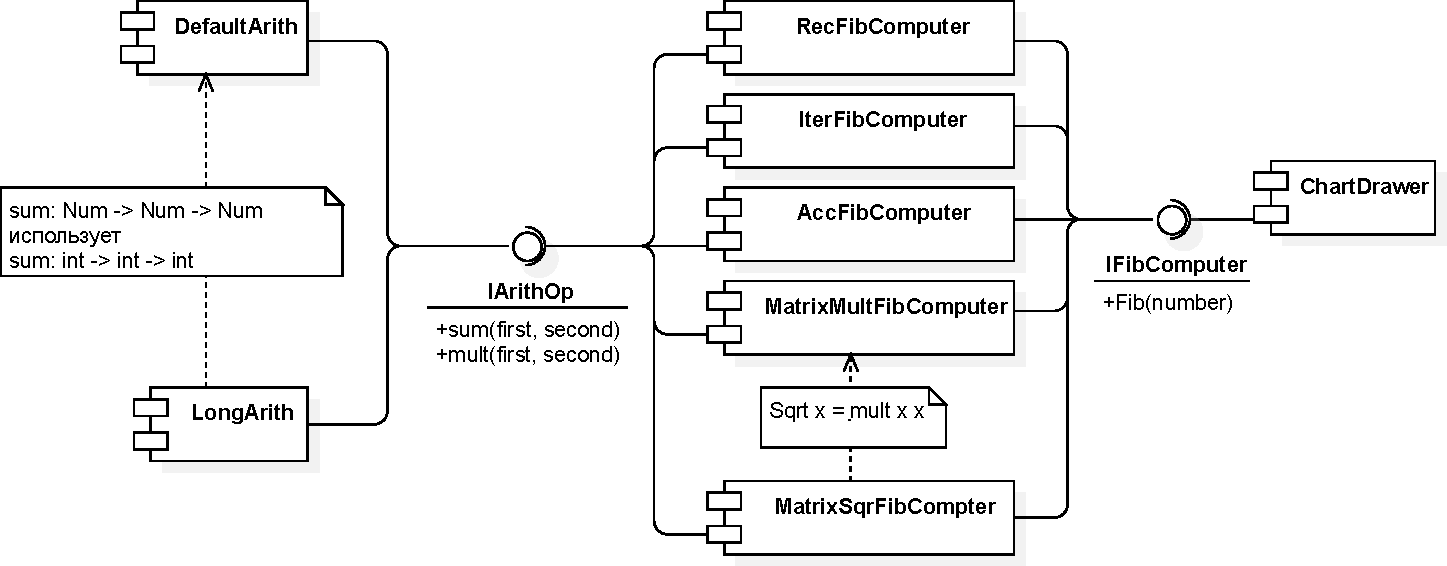
\includegraphics[width=1.25\textwidth]{DM}
\end{document}